\subsection{Partie préconditionneur}
La factorisation LU en algèbre linéaire dense est une méthode pour factoriser une matrice $A$ en deux matrices $L$ et $U$.
%
$L$ est une matrice triangulaire inférieure, toutes les valeurs au-dessus de la diagonale sont nulles.
%
Symétriquement, $U$ est une matrice triangulaire supérieure, toutes les valeurs de $U$ en-dessous de la diagonale sont nulles.
%
Le principal intérêt de cette factorisation est de trouver facilement $x$ dans les équations du type $Ax=y$.
%
Dans le cas où $A=L.U$, le système d'équations $Ax=y$ est transformée en deux systèmes d'équations $L.x_{tmp}=y$ et $U.x=x_{tmp}$.
%
La méthode utilisée pour résoudre les systèmes composés de matrices triangulaires est triviale.
%
Il suffit de résoudre chaque équation ligne par ligne en commençant par la ligne qui n'a qu'une seule valeur non nulle.
%
Ensuite il faut résoudre la ligne avec deux valeurs non nulles dont une des inconnues provient de la solution précédente, et ainsi de suite jusqu'à la dernière ligne.
%
Il existe du parallélisme à exploiter dans cet algorithme, à chaque fois qu'une inconnue est trouvée, on peut la retirer de chacune des lignes restantes à traiter~\cite{plasma_lu}.



En algèbre linéaire creuse, la transformation des éléments nuls de la matrice creuse en éléments non nuls est appelée remplissage.
%
La factorisation LU d'une matrice $A$ creuse donnera deux matrices triangulaires denses $L$ et $U$.
%
Or, si l'on souhaite effectuer la factorisation exacte dans le cas d'une matrice d'ordre élevé ($>$ 100 000), ces deux matrices ne peuvent pas tenir en mémoire.
%
C'est pourquoi en algèbre linéaire creuse, on utilise une version altérée de cette factorisation que l'on appelle factorisation incomplète, ou {\em ILU}\footnote{Incomplete LU}, dont le but est de limiter le remplissage de la matrice.
%
En contrepartie, le résultat de la factorisation obtenu est approximatif et fournit donc un moins bon préconditionneur pour GMRES.
%
L'algorithme ILU est similaire à l'algorithme LU mais le remplissage est limité par des conditions définies par l'algorithme.
%
Ces conditions peuvent être de deux formes : soit en limitant le remplissage avec une valeur seuil (ILUT\cite{saad1994ilut}), soit en limitant le niveau d'interaction entre les lignes de la matrices (ILU(k)).
%
Dans le cas ILU(k), le paramètre k sert à limiter le niveau d'interaction entre les lignes.
%
Avec $k=0$, le motif des matrices $L$ et $U$ reste similaire au motif de la matrice $A$ (Algo~\ref{algo:ilu0}).
%
En augmentant la valeur de $k$, on augmente aussi le nombre d'interactions entre les cellules.





L'algorithme ILU offre la possibilité de factoriser certaines lignes en parallèle et ce parallélisme se représente naturellement sous la forme d'un graphe de tâches (Fig.~\ref{fig:example_3_dag}).
%
Chaque tâche représente la factorisation d'une ligne de la matrice et les dépendances entre les tâches sont données par le motif de la matrice.
%
En effet, pour factoriser la ligne $i$, nous devons factoriser toutes les lignes $j$ inférieures à $i$ tel que l'entrée $(i,j)$ de la matrice soit non nulle.
%
Cette dépendance de donnée provient de la ligne~\ref{algo:ilu0:dep} de l'algorithme~\ref{algo:ilu0}.
%
C'est cette dépendance qui nous empêche que d'utiliser du parallélisme de boucle pour paralléliser la méthode ILU.
%
Donc, à partir du motif des valeurs non-nulles de la matrice, nous pouvons facilement construire le graphe de tâche:
%
la tâche $i$ corresponds à la ligne $i$ de la matrice (ligne \ref{algo:ilu0:task_begin} à \ref{algo:ilu0:task_end} de l'algorithme~\ref{algo:ilu0}), la liste des tâches prédécesseurs de la tâche $i$ est donnée par l'index de colonne des valeurs non-nulles avant la diagonale dans la ligne $i$ (ligne~\ref{algo:ilu0:dep}) et la liste des tâches successeurs de la tâche $i$ est donnée par l'index de ligne des valeurs non-nulles au-dessous de la diagonale de la colonne $i$ (Fig.~\ref{fig:example_2_matrix}).

\begin{figure}[!h]
     \begin{center}
        \subfigure[Un réservoir à 4 cellules]{
          \label{fig:example_1_res}
          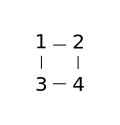
\includegraphics[width=0.30\textwidth]{example_1_res}
        }
        ~
        \subfigure[Une matrice avec 4 cellules]{
          \label{fig:example_2_matrix}
          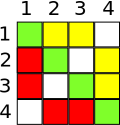
\includegraphics[width=0.30\textwidth]{example_2_matrix}
        }
        ~
        \subfigure[Un DAG à 4 cellules]{
          \label{fig:example_3_dag}
          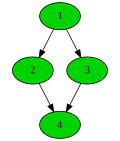
\includegraphics[width=0.30\textwidth]{example_3_dag}
        }
    \end{center}
    \caption{Trois représentations d'un réservoir. Les éléments en rouge dans la matrice déterminent les dépendances dans le graphe de tâches.}
    \label{fig:exemple_3_dag}
\end{figure}

\begin{algorithm}
  \KwData{$M$ : matrice de dimension $n$}
  \For{$i = 2$ {\bf à} $n$} {
    \For{$k = 1$ {\bf à} $i - 1$ {\bf et} $M_{ik} != 0$} { \label{algo:ilu0:task_begin}
      $M_{ik} = M_{ik} / M_{kk}$ \label{algo:ilu0:dep}\\
      \For{$j = k + 1$ {\bf à} $n$ {\bf et} $M_{ij} != 0$} {
        $M_{ij} = M_{ij} - M_{ik}M_{kj}$ \\
      }
    } \label{algo:ilu0:task_end}
  }
  \caption{Factorisation ILU(0) sur place.}
  \label{algo:ilu0}
\end{algorithm}


En résumé, le parallélisme de l'algorithme ILU peut se représenter sous la forme d'un graphe de tâches.
%
Chaque tâche représentant la factorisation d'une ligne... ce qui représente peu de calculs.
%
En fait, la plupart des runtimes mettront plus de temps à ordonnancer la tâche que la tâche mettra à s'exécuter.


Les problèmes rencontrés pour paralléliser la factorisation incomplète d'une matrice creuse, ainsi que les résolutions triangulaires associées, sont des problèmes qui représentent bien la difficulté que l'on peut rencontrer avec une parallélisation à grain fin.
%
La description à grain fin de ces algorithmes est naturelle, mais en pratique, une simple parallélisation utilisant des ordonnanceurs répandus, tels que Intel TBB ou OpenMP, ne donnera pas de bonnes performances à cause du faible coût de calcul d'une tâche.
%
Chaque ordonnanceur aura son propre algorithme de distribution des tâches qui prendra différents paramètres en compte.
%
Mais l'évaluation de cet algorithme coûte du temps et si ce temps est du même ordre de grandeur (ou plus grand) que le temps de calcul d'une tâche, l'ordonnanceur sera perçu comme une charge non désirée.
%
On appelle cela le problème de granularité.
%
Un ordonnanceur mettra de l'ordre de la centaine de nanosecondes à ordonnancer une tâche.
%
Pour que ce temps devienne négligeable, il faudrait que ce ne temps ne représente pas plus de 0,1~\% du temps de calcul d'une tâche.
%
Les tâches doivent donc durer de l'ordre de la centaine de microseconde.
%
Mais pour atteindre cette durée, les tâches doivent devenir plus grosses, nous devons factoriser plusieurs lignes à l'intérieur d'une tâche.
%
Mais le choix de ces lignes n'est pas trivial, il faut limiter l'impact sur le parallélisme et ne pas changer le résultat final.
%
Si trop de lignes à factoriser se retrouve dans une seule tâche, de nombreuses tâches devrons attendre que cette tâche finisse avec de pouvoir être exécuter même si les lignes dont elles dépendent sont déjà factorisées, nous avons donc détruit du parallélisme.
%
Un intergiciel a été développé dans cette thèse pour résoudre ce problème de manière transparente pour le programmeur.



De plus, l'ordre de factorisation des lignes de la matrice aura une influence sur les performances.
%
En fonction du nombre de variables primaires, nous avons entre 24~\% et 450~\% de temps de factorisation en plus par rapport au temps de factorisation optimal (Tab.~\ref{tab:facto_order}).
%
La factorisation des lignes de la matrice avec un parcourt linéaire des indices donne les meilleurs performances.
%
Les lignes consécutives de la matrice correspondent la plupart du temps à des cellules proches qui auront donc des interactions entres elles.
%
La factorisation d'une ligne utilisera donc souvent une partie du résultat de la factorisation de la ligne précédente, ce résultat ayant de grande chance d'être encore en mémoire cache.
%
Il est donc primordial d'agréger des tâches qui factorisent des lignes consécutives de la matrice.


%   (-_-)   %
\begin{center}
  \begin{tabular}{|r|c|c|c|}
    \hline
    Nombre de variables primaire & Temps avec un parcourt & Temps avec un parcourt & Pourcentage de temps\\
    & linéaire des indices (s) & non linéaire des indices (s) & en plus \\
    \hline
    1 & 0.16 & 0.88 & 450~\% \\
    \hline
    3 & 0.43 & 1.43 & 230~\% \\
    \hline
    8 & 3.95 & 5.18 & 24~\% \\
    \hline
  \end{tabular}
  \captionof{table}{Différence de temps d'une factorisation d'une matrice de 1 million de lignes en fonction de la méthode de parcours des indices de lignes.}
  \label{tab:facto_order}
\end{center}




Il existe des travaux de recherche dont le but est aussi d'exploiter le parallélisme de l'algorithme ILU :
%
En changeant la numérotation des cellules, on peut modifier la structure de la matrice ce qui aura pour effet de changer la factorisation.
%
Une renumérotation rouge-noire permet de factoriser parallèlement la moitié des lignes de la matrice dans un premier temps, puis la seconde moitié des lignes dans un second temps.
%
Cette technique offre énormément de parallélisme mais aura un impact négatif sur la convergence\cite{red_black_ilu}.
%
Plus récemment, une autre méthode a été développée permettant de factoriser tous les éléments de la matrice en parallèle tout en gardant une numérotation naturelle.
%
L'opération de factorisation parallèle est appelé {\em sweep} et doit être effectuée plusieurs fois\cite{chow2014fine}.
%
En moyenne 3 sweeps suffisent à obtenir un résultat proche de la factorisation incomplète.
%
La convergence n'est donc que faiblement dégradée, mais il faut prendre en compte que 3 sweeps ont été nécessaires et il a donc fallu faire 3 fois plus d'opérations qu'une factorisation ILU classique.
%
Dans notre cas, nous nous intéressons à des renumérotation qui favorise le regroupement des tâches mais ne changent pas le résultat numérique.


%   (-_-)   %
\begin{figure}[!h]
     \begin{center}
        \subfigure[Exemple de graphe de tâche obtenu avec une numérotation naturelle.]{%
          \label{fig:DAG_natural}
          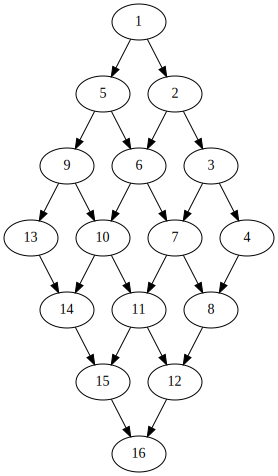
\includegraphics[width=0.33\textwidth]{DAG_natural}
        }%
        \subfigure[Exemple de graphe de tâche obtenu avec une numérotation rouge-noire.]{%
          \label{fig:DAG_redblack}
          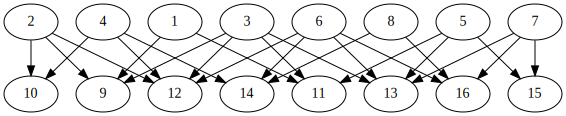
\includegraphics[width=0.66\textwidth]{DAG_redblack}
        }%
    \end{center}
    \caption{Différence de parallélisme en fonction de la numérotation choisie. La figure \ref{fig:matrix_ordering} représente les matrices associées.}
    \label{fig:DAG_ordering}
\end{figure}
